
\section{Dipol Antenne}\label{sec:DipolAntenne}
Der zentral gespiesene Dipol besteht oft aus zwei runden Leiterstäben mit dem Durchmesser $d$ und der Länge $l$. Die beiden Stäbe haben eine gesamte Länge von $2l$ und liegen bis auf eine kleine Lücke direkt hintereinander. Die gesamte Länge der beiden Stäbe ist viel grösser als der Durchmesser $d$. Wird eine Spannung in der Lücke zwischen den beiden Stäben angelegt, kommt es zu einer Stromverteilung über die gesamte Länge. Oft wird die Spannung mit einer Zweidrahtleitung,  diese wird englisch \textit{Transmission Line} genannt, zwischen den Leiterstäben angebracht. Die anschliessende Stromverteilung entlang der beiden runden Leiterstäbe liefert den Ursprung der Wellenausbreitung. In einer ersten Näherung kann die sich von der Speisestelle ausbreitende Welle als richtungsunabhängige Kugelwelle betrachtet werden mit folgender mathematischer Beschreibung: \cite{elliott1981antenna}.
%E^j(wt-kr)/4pimu^-1 r
%Elliot Seite 29 Nr1.93

\begin{equation}\label{term:Kugelwelle}
\frac{e^{j(\omega t-kr)}}{4\pi \mu_{0}^{-1}r}
\end{equation}


%%%%%%%%%%%%%%%%%%%%%%%%%%%%%%%%%%%%%%%%%%%%%%%%%%%%%%%%%%%%%%%%%%%
\begin{figure}[!ht]
	\centering
	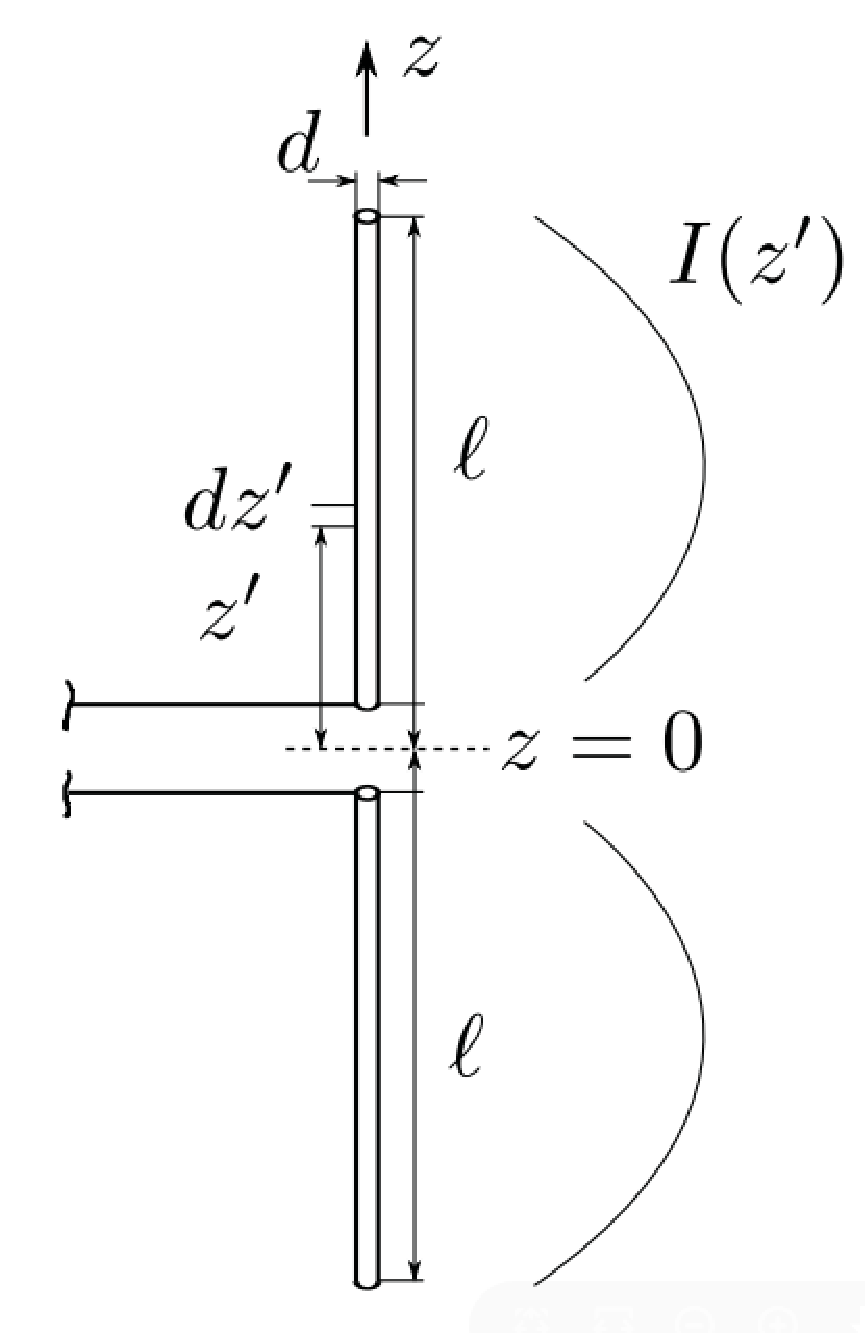
\includegraphics[width=4cm]{content/bilder/Dipol_EMANT_S42.pdf}%
	\caption{Dipol Antenne mit Stromverteilung \cite{Tekom}}
	\label{FitzDipol}
\end{figure}
%%%%%%%%%%%%%%%%%%%%%%%%%%%%%%%%%%%%%%%%%%%%%%%%%%%%%%%%%%%%%%%%%%%
Die Dipol Antenne entspricht einer Zweidrahtleitung mit offenen, um $90^\circ$ abgewinkelten Drahtarmen. Die offenen Enden der Dipolarme führen zu einer Reflexion der zuführenden Spannungswelle in die umgekehrte Richtung und somit zu einer stehenden Welle. Stromführende Elemente, welche nahe beieinander liegen und deren Stromamplituden betragsmässig gleich, jedoch entgegengesetzt sind, strahlen nur gering. Dies trifft auf die Zuführung der Dipol Antenne zu. Die voneinander abgewinkelten Dipolarme strahlen jedoch stark, da aufgrund des durch die räumliche Trennung entstehenden elektrischen Feldes elektromagnetische Wellen abgestrahlt werden.
Als Näherung für die Stromverteilung in den Dipolarmen soll Folgendes gelten \cite{elliott1981antenna}:
\begin{equation}\label{I_xt_Dipol} 
I(x,t) =I_{m}sin([k(l-x)])e^{j\omega t}
\end{equation}
%Elliot Seite 59 Formel 2.1

Aus  (\ref{I_xt_Dipol}) kann entnommen werden, dass sich der Strom entlang der Dipolarmen ändert. Die Stromverteilung ist somit vom Betrachtungsort $x$ und dem Zeitpunkt $t$ abhängig. Ein Dipol mit einem Durchmesser $d<<\lambda$ wird  zu einem dünnen Stromfaden, welcher nur eine Ausdehnung entlang der z-Achse aufweist. Die Stromdichte im Leiter $J \textit{d}V$ kann daher mit $I\textit{d}l$ ersetzt werden. Werden die Arme des Dipols in sehr viele kurze Stücke $\textit{\textit{d}}z$ geteilt, so entsprechen diese jeweils einem Hertzschen Elementardipol mit konstanter Stromdichte. Sowohl die Elementardipole als auch deren Summe können als punktförmige Quelle elektromagnetischer Wellen betrachtet werden. Die Gewichtsfunktion $a(\varphi)$ dieser Summe lautet: \cite{elliott1981antenna}.\\

\begin{equation}
I(z')=I_{m}sin(k(l-dz))
\end{equation}
%Elliot Seite 61 Formel 2.2

\begin{equation}
a(\varphi)= 0
\end{equation}
Die Gewichtungsfunktion in Abhängigkeit von $\theta$ beträgt nach folgender Formel (\ref{eq:Gewichtungsfunktion}) \cite{elliott1981antenna}:
\begin{equation}\label{eq:Gewichtungsfunktion}
a_{\theta}(\theta)=- \frac{2I_{m}}{k sin(\theta)} \Big\lbrack cos(kl cos(\theta)) - cos(kl) \Big\rbrack
\end{equation}
%Elliot Formel 2.6 oder Joss EMANT 122.
Es sollen nun zwei Spezialfälle einer Dipol Antenne genauer betrachtet werden:
\begin{itemize}
\item der Halbwellendipol mit 2l = $\lambda/2$
\item der kurze Dipol mit 2l$ \ <<\lambda$
\end{itemize}
\newpage
\subsubsection{Halbwellendipol 2l = $\lambda/2$}
Der $\lambda/2$-Dipol ist eine der wichtigsten Antennen. Über die Gewichtungsfunktion in Formel (\ref{eq:Gewichtungsfunktion}) und den Term der sich ausbreitenden Kugelwelle aus (\ref{term:Kugelwelle}) lässt sich auf das Fernfeldverhalten des Halbwellendipols schliessen \cite{elliott1981antenna}:\\
\begin{equation}
E_{\theta}=j60I_{m} \frac{e^{j(\omega t - kr)}}{r} \biggl\lbrack \frac{  (\pi/2) cos(\theta)\rbrack}{sin(\theta)} \biggr\rbrack
\end{equation}
\begin{equation}
H_{\phi}=j \frac{I_{m}}{2\pi} \frac{e^{j(\omega t - kr)}}{r} \biggl\lbrack \frac{cos\lbrack  (\pi/2) cos(\theta)\rbrack}{sin(\theta)} \biggr\rbrack
\end{equation}\\
%E(theta)= Ellito 2.8
%E(phi) = Ellito 2.9
Die Feldverteilung einer Antenne kann in einem zwei- oder dreidimensionalen Richtdiagramm dargestellt werden. Die nachfolgende Abbildung \ref{fig:DipolEFerd} zeigt die E-Feldverteilung eines $\lambda/2$-Dipols, ausgerichtet entlang der z-Achse, in der xz-Ebene mit Schnitt durch den Koordinatenursprung.\\



%%%%%%%%%%%%%%%%%%%%%%%%%%%%%%%%%%%%%%%%%%%%%%%%%%%%%%%%%%%%%%%%%%%
\begin{figure}[!ht]
\begin{center}
\begin{tikzpicture}
	\draw (0,3)  -- (10,3);%Fadenkreuz horizontal node at (0.5,0.5) {xz Ebene}
	\draw (5,0) -- (5,6);%Fadenkreuz vertikal
	\draw [line width=1mm] (5,3.2) -- (5,4.5);%upper arm
	\draw [line width=1mm] (5,1.5) -- (5,2.8);%lower arm
	\draw (3,3) circle (2cm);%linker Kreis
	\draw (7,3) circle (2cm);%rechter Kreis

	\node[draw] at (5,6.5) {$\theta=0 ^\circ$};
	\node[draw] at (8,5.5) {$E(\theta)$};
	
	\draw[line width=0.4pt, ->, >=latex](5, 5) -- (5, 6.1) node at (4.5,6){z};
	\draw[line width=0.4pt, ->, >=latex](9, 3) -- (10.1, 3) node at (10.5,3){x};
	
	\draw[line width=0.4pt, ->, >=latex](5, 3) -- (7, 5) node at (7,4.7){$\vec{r}$};

	\coordinate (A) at (5, 5.5);
	\coordinate (B) at (6.4, 4.5);
	\coordinate (a) at (5.6, 5.4);
	\draw[line width=0.5pt, dashed, very thick,cap=round,->](A) .. controls (a) .. node[above] {$\theta$} (B);
\end{tikzpicture}
\end{center}
	\caption{Das E-Feld einer Dipol Antenne in der xz-Ebene}
	\label{fig:DipolEFerd}
\end{figure}
%%%%%%%%%%%%%%%%%%%%%%%%%%%%%%%%%%%%%%%%%%%%%%%%%%%%%%%%%%%%%%%%%%%
Es ist zu erkennen, dass bei $\theta = 0 ^\circ $  und $\theta = 180 ^\circ $ kein elektrisches Feld besteht. Stellt man sich die Grafik als um eine um die z-Achse rotierende Scheibe vor, so entsteht die aus R.Elliott \cite{{elliott1981antenna}} bekannte Torusform. Die dargestellte rotierende Feldverteilung beschreibt demnach in der xy-Ebene einen Winkel $\varphi$ von $0 ^\circ $ bis $360 ^\circ $.
Die von $\theta$ und $\varphi$ abhängige Leistung des elektromagnetischen Feldes an einem beliebigen Punkt im dreidimensionalen Raum ist gegeben durch \cite{elliott1981antenna}:
%P(theta,phi)= elliot2.10
\begin{equation}
P(\theta,\varphi)=\frac{2\eta I_{m}^{2}}{(4\pi r)^{2}}\Bigl\lbrack \frac{cos^{2}\lbrack  (\pi/2) cos(\theta)\rbrack}{sin^{2}(\theta)}\Bigr\rbrack
\end{equation}
%Durch Lösung des Doppelintegrals 
%Elliot Seite 63
Die abgestrahlte elektromagnetische Leistung aller Oberflächenpunkte ist anhand des Doppelintegrals über die Torusoberfläche gegeben \cite{Emant}:
\begin{equation}
P_{rad}=\int_0^{2\pi} \int_0^\pi P(\theta,\varphi)r^2\sin(\theta) d\theta d\varphi
\end{equation}
Durch Auflösen des Doppelintegrals über $\varphi$ von 0 bis $2\pi$ und $\theta$ von 0 bis $\pi$ erhält man als Leistung \cite{elliott1981antenna}:
\begin{equation}
P_{rad}=0.609 \frac{\eta I_{m}^{2}}{2\pi}
\end{equation}
%elliot 63 Forlmel 2.11
Wie aus Grafik \ref{fig:DipolEFerd} ebenfalls ersichtlich wird, liegt die maximale Feldausbreitung bei $\theta =\pm 90 ^\circ $, da $\sin(90^\circ)  $ = 1.
Der maximale Richtwert oder Richtfaktor des elektromagnetischen Feldes einer Antenne, aus dem englischen als \textit{directivity} $D$ bekannt, erhält man durch den Vergleich der von ihr abgestrahlten Leistung mit derjenigen eines isotropen Kugelstrahlers \cite{elliott1981antenna}:
\begin{equation}
D(peak)=\frac{P(\theta,\varphi)(\pi/2)}{P_{rad}/ 4 \pi r^{2}} =1.64
\label{eq:Directivity}
\end{equation}
%Dmax=1.64 nach Ellito 2.12
Der Richtwert von 1.64 besagt, dass das elektromagnetische Feld einer Halbwellenantenne im Raum nicht homogen ist. Er stellt einen Verhältnisfaktor dar, welcher sich auf einen gleichmässig in den Raum strahlenden Kugelstrahler bezieht. Die maximale Ausbreitungsrichtung des elektromagnetischen Feldes, auch Hauptkeule genannt, beschreibt die Richtung der grössten Abstrahlung. Sie ist bei einem Halbwellendipol um den Faktor 1.64 grösser als bei einem isotropen Kugelstrahler. Der Richtfaktor wird in der Einheit Dezibel dB angegeben. In Bezug auf den isotropen Strahler erfolgt die Angabe in der Einheit dBi. Der Richtfaktor entspricht in dem gezeigten Beispiel (\ref{eq:Directivity}) $10\log{(1.64)}=2.15$ dBi.\\

Bei einem Halbwellendipol der Länge 2l mit $l=\lambda/4 $ ist der Scheitelwert des Antennenstromes $I_{m}$ beim Einspeisepunkt. Dieser liegt im Zentrum des Dipols bei z = 0. Somit kann gesagt werden, dass die Zuleitung die folgende Leistung liefert \cite{Emant}:
%Elliot 2.14
\begin{equation}
P=\frac{1}{2} I_{m}^{2}R_{rad}=(0.609)\frac{\eta I_{m}^{2}}{2\pi}
\end{equation}
Der Strahlungswiderstand, auch $R_{rad}$ genannt, kann im Falle des $\lambda /2$-Dipols nummerisch als 73 Ohm bestimmt werden.
\begin{equation}\label{RradDipol}
R_{rad}=\frac{0.609 \eta}{\pi}= 73 \ Ohm
\end{equation}
